\chapter{Retractos}%
\label{cha:retractos}
\section{Retractos y deformaciones}%
\label{sec:retractos_y_deformaciones}
\begin{defi}
Una aplicación $\rho: X \rightarrow A \subset X$ es:
\begin{enumerate}
    \item Un \underline{retracto} si $\rho|_A = id_A$ (y $A = \rho\left( A \right)$ es un \underline{retracto de $X$})
    \item Una \underline{deformación} (fuerte) si: $\exists H_s: id_X \stackrel{A}{\simeq} \rho$, homotopía relativa a $A$.
\end{enumerate}
\end{defi}

\begin{ej}
\begin{enumerate}
    \item $\forall$ cte $: X \rightarrow \{x_0\} \subset X$ es retracto.
    \item El retracto \underline{radial} $\rho: \mathbb{R}^{n + 1} \setminus \{0\} \rightarrow \mathbb{S}^n: x \mapsto x / \lVert x \rVert$ es una deformación. $H_s\left( x \right) = \left( 1 - s \right) x + s\rho\left( x \right)$.
    \item $\begin{rcases}
        \rho: X \rightarrow A \subset X \subset \mathbb{R}^n \text{ retracto}\\
        \left[ x, \rho\left( x \right) \right] \subset X,\ \forall x
    \end{rcases} \Rightarrow \rho$ deformación: $H_s = \left( 1 - s \right) id_X + s\rho$ (interpolación).
    \item Cilindros: 
    \begin{align*}
        \rho: X \times \left[ 0, 1 \right] &\rightarrow X \times \{0\}\\
        \left( x, t \right) &\mapsto \left( x, 0 \right) = \rho \left( x, t \right) 
    .\end{align*}
    con $\rho$ deformación sobre $X : H_s\left( x, t \right) = \left( x, \underbrace{\left( 1 - s \right) t}_{\left( 1 - s \right) t + s \cdot 0} \right)$.
    %TODO: Imagen
    \begin{center}
        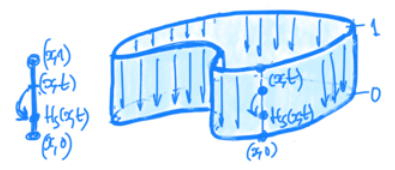
\includegraphics[scale=0.3]{images/deformacion_cilindros} 
    \end{center}
    \item Banda de Möbius: $\mathbb{S}^1 \subset M = \bigcup_{p \in \mathbb{S}^1} \left[ a_p, b_p \right]$.

    Deformación sobre $\mathbb{S}^1: \begin{cases}
        \rho: M \rightarrow \mathbb{S}^1: x \mapsto \rho\left( x \right)\\
        H_s\left( x, s \right) = \left( 1 - s \right) x + s\rho\left( x \right) 
    \end{cases}$
    %TODO: Imagen
    \begin{center}
        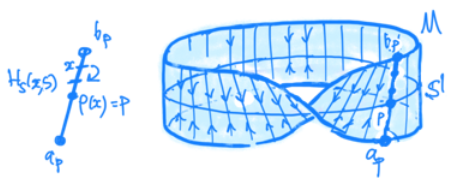
\includegraphics[scale=0.3]{images/deformacion_moebius} 
    \end{center}
\end{enumerate}
\end{ej}

\begin{prop}
Sea $\rho: X \rightarrow A \subset X,\ a_0 \in A;\ \rho_*: \pi\left( X, a_0 \right) \rightarrow \pi\left( A, a_0 \right)$.
\begin{enumerate}
    \item $\rho$ retracto $\Rightarrow \rho_*$ suprayectivo.
    \item $\rho$ deformación $\Rightarrow \rho_*$ isomorfismo.
\end{enumerate}
\end{prop}
\begin{demo}
\begin{enumerate}
    \item $\rho$ retracto:
    %TODO: Imagen
    \begin{center}
        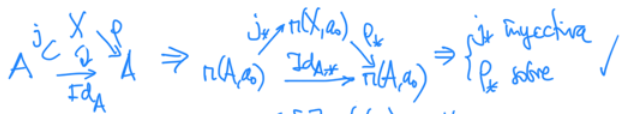
\includegraphics[scale=0.3]{images/dem_retracto_sobre} 
    \end{center}

    \item $\rho$ deformación:
    \[
    H_s: id_X \stackrel{A}{\simeq} \rho \Rightarrow j_* \text{ sobre.} : \begin{cases}
        \left[ \sigma \right] \in \pi\left( X, a_0 \right) &\Rightarrow H_s \circ \sigma: \sigma \stackrel{A}{\simeq} \rho \circ \sigma = j \circ \rho \circ \sigma\\
           &\Rightarrow \left[ \sigma \right] = \left[ j \circ \rho \circ \sigma \right] = j_*\left[ \rho \circ \sigma \right] 
    \end{cases} 
    \]
    y por ser $j_*$ sobre $\Rightarrow \rho_*$ inyectiva.
\end{enumerate}
\end{demo}

\begin{ej}
\begin{enumerate}
    \item $\pi\left( \mathbb{R}^{n + 1?} \setminus \{0\} \right) = \pi\left( \mathbb{S}^n \right) = \begin{cases}
        \{1\},\ n\ge 2\\
        \mathbb{Z},\ n = 1
    \end{cases}$
    \item $\pi$(cilindro) = $\pi$(banda de Möbius) $= \pi \left( \mathbb{S}^1 \right) = \mathbb{Z}$.
\end{enumerate}
\begin{demo}
    Veremos $\mathbb{S}^1$...
\end{demo}
\end{ej}

\section{Cocientes}%
\label{sec:cocientes}
Muchos espacios son cocientes y las deformaciones se pueden hacer compatibles para facilitar las construcciones.

\begin{ej}
Cilindro $C = \mathbb{S}^1 \times \left[ 0, 1 \right]$ y banda de Möbius $M$.
%TODO: Imagen
\begin{center}
    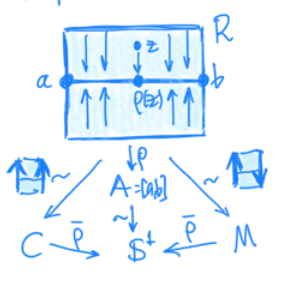
\includegraphics[scale=0.3]{images/coc_cilindro_moebius} 
\end{center}
Tenemos $C, M = R / $ identificaciones adecuadas de lados opuestos y, por otro lado, la deformación de $R$ sobre $A = \left[ a, b \right],\ H_s\left( z \right) = \left( 1 - s \right) z + s \rho\left( z \right) \xRightarrow{(*)}$ deformación de $R / \sim$ sobre $\left[ a, b \right] / \sim = \mathbb{S}^1$. 

Es decir, \fbox{$\mathbb{S}^1$ es deformación de $C$ y de $M$, luego todos tienen $\pi = \mathbb{Z}$.} 

$(*)$: porque $p$ y $H_s$ son \underline{compatibles con las relaciones}: $z \sim z' \Rightarrow H_s\left( z \right) \simeq H_s\left( z' \right)$, luego inducen aplicaciones continuas $\overline{\rho}$ y $\overline{H_s}: R / \sim\ \rightarrow A / \sim$. 

Normalmente se hacen las deformaciones pensando en que cumplan $H_s\left( z \right) \simeq H_s\left( z' \right)$.
\end{ej}

\section{Agujeros}%
\label{sec:agujeros}
Conviene insistir en un ejemplo importante de deformación y sus variantes.
%TODO: No sé que entorno usar aquí
\begin{enumerate}
    \item $\rho: \underbrace{\mathbb{R}^{n + 1} \setminus \{0\}}_{\text{esp. con ``agujero''}}  \rightarrow \mathbb{S}^n$ deformación $\Rightarrow \pi\left( \mathbb{R}^{n + 1} \setminus \{0\}, x_0 \right) =$ \[
    = \begin{cases}
        \mathbb{Z},\ n = 1 \text{ (se verá...)}\\
        \{1\},\ n \ge 2\ (\mathbb{S}^n,\ n \ge 2 \text{ simple-conexa}) 
    \end{cases} 
    \]

    \item Dibujos en $\mathbb{R}^2 \setminus \{c\}$ de retracciones sobre curvas ``alrededor'' del ``agujero'' $c$:
    %TODO: Imagen
    \begin{center}
        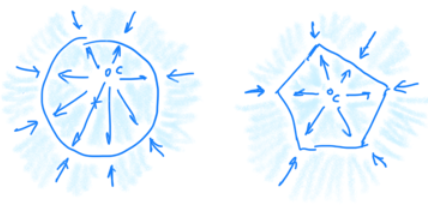
\includegraphics[scale=0.3]{images/curvas_R2_agujero_c} 
    \end{center}

    \item Dos agujeros $\mathbb{R}^2 \setminus \{a, b\}$.

    Se trocea el espacio en cerrados, en cada uno de los cuáles se hace una deformación, de manera que en las fronteras coincidan. En el dibujo se sombrean diferentes las zonas en las que se usan deformaciones diferentes. Las deformaciones más cómodas son las interpolaciones de $id$ y una retracción geométrica.
    %TODO: Imagen
    \begin{center}
        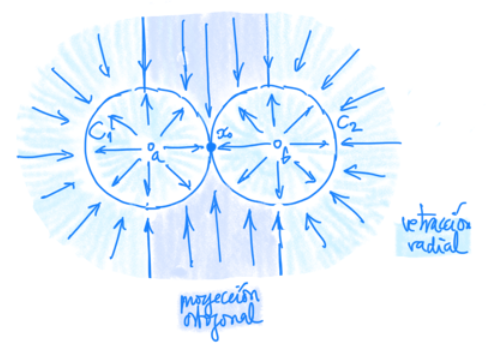
\includegraphics[scale=0.3]{images/curvas_R2_dos_agujeros} 
    \end{center}
    En este caso, $\rho: \mathbb{R}^2 \setminus \{a, b\} \rightarrow \infty?$ es deformación y $\pi\left( \mathbb{R}^2 \setminus \{a, b\}, x_0 \right) = \pi\left( \infty? \right) = \mathbb{Z} * \mathbb{Z}$ (grupo fundamental de una lemniscata).

    \item Otra variante:
    %TODO: Imagen
    \begin{center}
        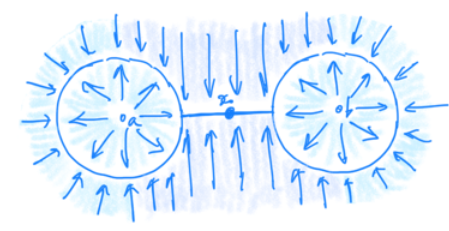
\includegraphics[scale=0.3]{images/variante_4_agujeros} 
    \end{center}
    %TODO
    $\mathbb{R}^2 \setminus \{a, b\} \rightarrow dibujo$ deformación dice que:
    \[
    \pi\left( dibujo \right) = \pi\left( \mathbb{R}^2 \setminus \{a, b\}, x_0 \right) = \pi \underbrace{\left( \infty? \right)}_{= \mathbb{Z} * \mathbb{Z}}  
    \]
    que es igual al grupo fundamental, pero \underline{no} homeomorfismo.

    \item Aún más ejemplos así (ya sin especificar el punto base):
    \[
    \pi\left( \mathbb{R}^2 \setminus \{a, b, c\} \right) = \pi\left( dibujo \right) = \pi\left( dibujo \right) = \pi \left( dibujo \right) = \mathbb{Z} * \mathbb{Z} * \mathbb{Z}
    \]
    \begin{demo}[creo]
    Cualesquiera tres puntos en $\mathbb{R}^2$ se pueden recolocar con homeomorfismos para hacer, a partir de ellos, retracciones sobre las curvas dibujadas, \underline{no homeomorfas}. (?) 
    \end{demo}
\end{enumerate}

\underline{Ejercicio}: Deformar $\mathbb{R}\mathrm{P}^2 \setminus \{a\}$ sobre una circunferencia, para obtener $\pi\left( \mathbb{R}\mathrm{P}^2 \setminus \{a\} \right) = \mathbb{Z}$.

